\documentclass[12pt,a4paper,twoside,index=totoc,listof=totoc,headinclude,headsepline,numbers=noenddot,headings=normal,parskip=half,fleqn]{scrbook}

%***********************************************************
%* Pakete			 									   *
%***********************************************************
\usepackage[utf8]{inputenc}       % Cross Platform
\usepackage[ngerman]{babel}       % Sprache: deutsch
\usepackage[babel,german=quotes]{csquotes} % Paket zur Silbentrennung und deutsche Anführungszeichen
\usepackage[left=2.7cm,right=2.7cm,top=3cm,bottom=3cm]{geometry}
\usepackage[dvipsnames]{xcolor}
\usepackage{graphicx}
\usepackage{tabularx}
                                    
\usepackage{siunitx}
\sisetup{
  locale = DE ,
  per-mode = fraction
}
\usepackage{float}              

\usepackage{enumitem}

\author{Cay Jakob Rahn}

\usepackage[headsepline]{scrlayer-scrpage}
\usepackage{scrhack}
\usepackage{color}
\usepackage{setspace}
\usepackage{longtable}
\usepackage{listings}
\usepackage{rotating}
\usepackage{pdfpages}
\parindent 0pt
\usepackage{booktabs}
\usepackage[export]{adjustbox}


%***********************************************************
%* Zitierstil											   *
%***********************************************************
\usepackage[backend=biber,
citestyle=authoryear-comp,
bibstyle=authoryear,
hyperref=true,
isbn=false,
doi=false
]{biblatex}
\setlength\bibitemsep{0.5\baselineskip}
\addbibresource{./bib/quellen.bib}
\ExecuteBibliographyOptions{maxcitenames=1,mincitenames=1}
%\DeclareLanguageMapping{ngerman}{german-apa}
\DefineBibliographyStrings{ngerman}{ 
   andothers = {{et\,al\adddot}},             
}

%***********************************************************
%* Schriftart		 									   *
%***********************************************************
\usepackage{mathptmx}
\usepackage[T1]{fontenc} % Paket zur Silbentrennung
\setkomafont{disposition}{\normalfont\bfseries} % Überschriften mit Serifen

% Abstand zwischen Kopfzeile und Kapitelüberschrift
%\renewcommand*{\chapterheadstartvskip}{\vspace*{.75\baselineskip}}

%***********************************************************
%* Formeln			 									   *
%***********************************************************
\usepackage{amsmath}
\usepackage{amsfonts}
\usepackage{amssymb}
\setlength{\mathindent}{3cm} % Einrücktiefe

%***********************************************************
%* Quellcode / Kommandozeileneingabe						   *
%***********************************************************
\lstdefinestyle{BashInputStyle}{
  language=bash,
  basicstyle=\small\ttfamily,
  frame=tb,
  columns=fullflexible,
  linewidth=0.9\linewidth,
  xleftmargin=0.1\linewidth
}

\usepackage[]{acronym}

\usepackage[hidelinks]{hyperref}
%***********************************************************
%* Beginn des Dokuments 									   *
%***********************************************************
\begin{document}
\begin{sloppypar}
\setstretch{1.2}

\frontmatter
\begin{titlepage}

	\thispagestyle{empty}
	\newgeometry{left=0cm, right=0cm, top=0.6cm, bottom=0cm, includefoot}
	
	% FH Logo
	\begin{flushright}
		
\includegraphics[width=1.7cm]{./pic/FHAC.jpg}
	\end{flushright}
	
	\vspace{-2.5cm}

	% Kopfzeile mit Fachbereich ...
	\centering \begin{bfseries} \Large Fachhochschule Aachen\\ \end{bfseries}

	\vspace{1.5cm}
	\normalsize
	Fachbereich 9\\
	Medizintechnik und Technomathematik
	
	\vspace{0.5cm}
	
	\centering \rule{0.75\textwidth}{1pt}
	
	\vspace{1cm}

	%Titel der Arbeit
	\centering \begin{minipage}[t]{17cm}
		\centering \bfseries \huge Hier\\Titel einfügen		\medskip
	\end{minipage}

	\vspace{1cm}
	
	\centering \rule{0.75\textwidth}{1pt}
	
	\vspace{1cm}
	
	
	\centering \textbf{Bachelorarbeit}\\
	\centering im Studiengang Scientific Programming

	\vspace{1cm}

	%Name und Matrikelnummer
	\begin{minipage}[t]{9cm}
		\centering \textbf{Cay Jakob Rahn} \\ \centering Matr.-Nr.: 3145495
	\end{minipage}
	
	\vspace{1cm}
	
	\begin{minipage}[b]{4cm}
		\centering \today
	\end{minipage}


	\vspace{2cm}

	%Prüfer
	\begin{minipage}[t]{10cm}
		\centering \begin{tabular}{ll}
		1. Prüfer: & Prof. Dr. rer. nat. Alexander Voß\\
		2. Prüfer: & Dr.-Ing. Christoph Hoog Antink
		\end{tabular}
	\end{minipage}


	\vspace{2cm}

	% Firmenlogo
	\begin{flushleft}
	\centering \hspace{-3cm}
	\begin{minipage}[t]{5cm}
			
\includegraphics[width=9cm]{./pic/Logo_MedIT_RWTH.png}
	\end{minipage}
	\end{flushleft}
	\restoregeometry


\end{titlepage}
\clearpage
\clearpage
\chapter*{Erklärung}\label{erklaerung}
\thispagestyle{empty}

Diese Arbeit ist von mir selbständig angefertigt und verfasst. Es sind keine anderen als die angegebenen Quellen und Hilfsmittel benutzt worden.

     
\vspace{1cm}

\begin{tabularx}{\textwidth}{lXl}
  \rule{5cm}{0.4pt} & & \rule{5cm}{0.4pt}\\
  Ort, Datum & & Unterschrift
\end{tabularx}

\clearpage
\clearpage
\chapter*{Abstract}\label{abstract}


Ballistokardiographie (BKG) ist eine Messtechnik, bei der die durch den Herzschlag induzierten Massenverschiebungen des Körpers gemessen werden. Störungen, sogenannte Artefakte, die diese Signale überlagern, führen zu Fehlern in der Signalverarbeitung und so womöglich zu fehlerhaften Diagnosen. Die Beurteilung der Signalqualität und damit die zuverlässige Detektion dieser Artefakte ist ein für das BKG bis jetzt nicht hinreichend gelöstes Problem, besonders bei in Betten integrierten BKG-Systemen. 

In dieser Arbeit werden die Grundlagen der Ballistokardiographie erarbeitet - der physiologische Ursprung, die Eigenschaften der Signale und Techniken der Signalverarbeitung. Messdaten werden aufbereitet und Methoden zur Beurteilung der Signalqualität, die sich für andere Aufnahmebedingungen erfolgreich zeigten, evaluiert. Aufbauend auf diesen Ergebnissen werden Merkmale entwickelt, die Informationen über die Signalqualität enthalten. Modelle maschinellen Lernens werden ausgewählt und für Besonderheiten der Daten erweitert.

Abschließend wird die Güte dieser Modelle bewertet und gezeigt, dass die Beurteilung der Signalqualität verbessert werden kann und sich diese Ergebnisse sogar auch auf andere Aufnahmesituationen übertragen lassen.



%***********************************************************
%* Inhaltsverzeichnis 									   *
%***********************************************************
\cleardoublepage
\setstretch{1.15}
\tableofcontents
\setstretch{1.2}
%***********************************************************
%* Abkürzungsverzeichnis 								   *
%***********************************************************
\clearpage
\chapter{Abkürzungsverzeichnis}\label{abkuerzungsverzeichnis}
\begin{acronym}[CART]
	\acro{AUC}{Area under the ROC Curve}
	\acro{CART}{Classification And Regression Trees}
	\acro{CLIE}{Continuous Local Interval Estimator}
	\acro{BKG}{Ballistokardiographie}
	\acro{DT}{Decision Tree}
	\acro{EKG}{Elektrokardiographie}
	\acro{FPR}{False Positive Rate}
	\acro{HR}{Herzrate}
	\acro{HRV}{Herzratenvariabilität}
	\acro{LDA}{Linear Discriminant Analysis}
	\acro{MAE}{Mean Absolute Error}
	\acro{MSE}{Mean Squared Error}
	\acro{MLP}{Multilayer-Perzeptron}
	\acro{PCA}{Principal Component Analysis}
	\acro{PPG}{Photoplethysmographie}
	\acro{RF}{Random Forest}
	\acro{ROC}{Receiver Operating Characteristic}
	\acro{SKG}{Seismokardiographie}
	\acro{SQI}{Signal Quality Index}
	\acroplural{SQI}[SQIs]{Signal Quality Indices}
	\acro{SVM}{Support Vector Machine}
	\acro{TPR}{True Positive Rate}
	\acro{XGB}{eXtreme Gradient Boosting}
\end{acronym}


%***********************************************************
%* Abbildungssverzeichnis 								   *
%***********************************************************
\listoffigures

%***********************************************************
%* Tabellensverzeichnis  								   *
%***********************************************************
%\clearpage
%\listoftables

%***********************************************************
%* Hauptteil			 								   *
%***********************************************************
\clearpage
\setstretch{1.2}
%\raggedbottom % Abstandsabstände nicht variieren für vertikalen Ausgleich
% (alle letzten Zeilen auf einer Höhe)
\mainmatter

\chapter{Einleitung}\label{einleitung}

\section{Motivation}

Der derzeitige demographische Wandel stellt das Gesundheitssystem vor eine große Herausforderung: Immer mehr Patient*innen müssen im Alter überwacht und versorgt werden. Eine kontinuierliche autonome Überwachung von Vitalparametern im Krankenhaus oder auch Zuhause erlaubt es, Erkrankungen frühzeitig zu erkennen oder zu beobachten, ohne dass große Personalkapazitäten von Nöten sind.

Für diesen Anwendungszweck eignen sich vor allem Messmethoden, die die Patient*innen im Alltag nicht einschränken und wenig invasiv sind. Im Englischen wird dies mit dem Begriff \textit{unobtrusive} bezeichnet. Da es keine zufriedenstellende deutsche Entsprechung gibt, wird dieser im Folgenden nicht übersetzt verwendet werden. Solche \textit{unobtrusive} Messmethoden beinhalten meist keine Notwendigkeit für direkten Körper- oder Hautkontakt, liefern aber Information über Atmung und Herzschlag. Die Herausforderung bei so ermitteltem Signal besteht in der Signalverarbeitung, da Messungenauigkeiten und Alltagsbewegungen zu Störungen im Signal führen. Nicht informatives, also nicht für die Verarbeitung geeignetes Signal muss aber zwingend identifiziert werden, da die Ergebnisse stark verfälscht werden.

Eine solche \textit{unobtrusive} Messmethode ist die \acf{BKG}. Sensoren lassen sich beispielsweise in Betten und Stühlen implementieren. Aufgezeichnet werden Aktivitäten des Herzens und der Atmung. Die Signalmorphologie variiert jedoch sowohl zwischen den Patient*innen als auch innerhalb einer Person sehr stark, wodurch die automatische Beurteilung der Signalqualität erschwert wird. Um eine aussagekräftige Signalverarbeitung zu ermöglichen, ist dies jedoch essentiell. Besonders bei in Betten aufgenommenem Signal ist die Variation des Signals in Kombination mit Artefakten durch Körperbewegungen oder ähnliches problematisch.  
 

\section{Ziel der Arbeit}

Das Ziel dieser Arbeit ist es, Möglichkeiten der Beurteilung der Signalqualität von \ac{BKG}-Signalen mittels maschinellen Lernens zu untersuchen. Im besonderen Fokus liegen dabei Langzeitaufnahmen von bettlägerigen Patient*innen, da diese sich in der Vergangenheit als besonders anfällig für geringe Signalqualität gezeigt haben.

Dafür werden zunächst existierende Verfahren der Artefakterkennung für die vorliegenden Daten getestet und bewertet. Anschließend wird auf Basis von Domainenexpertise Merkmalskonstruktion betrieben und verschiedene Verfahren und Eingabeparameter verglichen. % TODO: was genau soll das Ergebnis sein?

Langfristig soll ermöglicht werden, \acf{BKG} im medizinischen Alltag anzuwenden. % TODO: sinnvoller schreiben

\textbf{To be continued}




\section{Gliederung}

\chapter{Grundlagen}\label{grundlagen}

Zum Verständnis dieser Arbeit ist grundlegendes Wissen nötig, welches hier in die drei Bereiche \nameref{ml-grundlagen}, \nameref{med-grundlagen} und \nameref{ballistokardiographie} unterteilt ist.


\section{Maschinelles Lernen}\label{ml-grundlagen}

Da in dieser Arbeit Methoden des Maschinellen Lernens verwendet werden, wird im Folgenden eine Übersicht über seine Prinzipien, gängige Techniken und Evaluationsmetriken sowie verschiedene Lernmodelle und deren mathematischen Hintergrund gegeben.

	\subsection{Grundprinzipien}
	
	Maschinelles Lernen ist die \glqq künstliche\grqq{} Generierung von Wissen auf Basis von Erfahrung: Aus Beispielen wird gelernt und dieses Wissen nach einer Trainingsphase verallgemeinert. Dafür wird mit Mustererkennung gearbeitet und ein statistisches Modell aufgebaut, das auf den Trainingsdaten beruht. Die Trainingsdaten $X$ bestehen aus Merkmalsvektoren $x \in X \subseteq \mathbb{R}^n$. %TODO: Hogi fragt was n ist
	Gesucht ist eine Funktion $f: X \to Y$, die diese Daten abbildet. Unterschieden wird bei der Beschreibung dieser Daten zwischen Klassifikation und Regression. Bei einer Klassifikation werden die Eingabedaten in verschiedene Klassen unterteilt. Bei einer Regression dagegen werden stetige Werte vorhergesagt, es wird die Verteilung der Daten beschrieben. Sie kann z.\,B. dafür genutzt werden, Verkaufszahlen vorauszusagen. Bei einigen Klassifikationsverfahren wird außerdem die Wahrscheinlichkeit der Angehörigkeit zu einer Klasse benannt.
	
	Es wird zwischen verschiedenen Arten des maschinellen Lernens unterschieden, dem überwachten und dem unüberwachten Lernen. Letzteres wird hier nicht betrachtet. Bei überwachtem Lernen bestehen die vorliegenden Daten aus Eingabe-Ausgabe-Paaren $(x_1, y_1), ...,(x_n, y_n) \text{ mit } x_i \in X \text{ und } y_i \in Y$. %TODO 3 punkte
	 Demnach ist nur die Funktion $f: X \to Y$ unbekannt. Der Lernalgorithmus sucht aus einem Hypothesenset die Funktion $g$, die $f$ möglichst gut approximiert. Ein Lernalgorithmus ermittelt diese Funktion aus einem Hypothesenset. Dieses Vorgehen ist in Abbildung\,\ref{fig:supervisedLearning} visualisiert. Bei unüberwachtem Lernen dagegen ist $Y$ unbekannt; die Eingabedaten haben die Form $x_1, ..., x_n \text{ mit } x_i \in X$. Hier ist ein $f$ gesucht, das die Daten möglichst gut beschreibt und sie beispielsweise eigenständig in Kategorien einteilt. In dieser Arbeit wird allerdings ausschließlich überwachtes Lernen betrachtet.
	
	\begin{figure}[H]
		\centering
		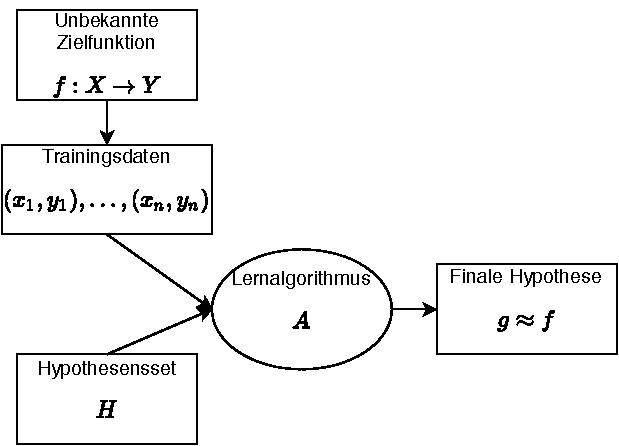
\includegraphics[scale=1]{pic/SupervisedLearning.pdf}
		\caption[Darstellung von überwachtem Lernen]{Darstellung von überwachtem Lernen}
		\label{fig:supervisedLearning}
	\end{figure}

	
	Ein häufig beobachtetes Problem bei maschinellem Lernen ist das sogenannte Overfitting, auf Deutsch Überanpassung, wenn das Modell zwar die Trainingsdaten gut approximiert, aber keine gute Generalisierung für unbekannte Daten bildet, d.\,h. zu stark an die Trainingsdaten angepasst ist. Gründe dafür können eine zu hohe Komplexität des Lernmodells wie z.\,B. zu viel Training oder zu wenig Trainingsdaten sein. %TODO: Satz fixen
	In beiden Fällen wird ungewollt ein Teil des \textit{noise} %TODO: evtl. einführen
	der Trainingsdaten in das Modell übernommen. Das Gegenteil von Overfitting ist Underfitting, das den Fall beschreibt, in dem das Modell die Beziehung von Merkmalen und Ziel nicht ausreichend erfasst. Dies ist unter anderem der Fall, wenn die zum Training verwendete Stichprobe verzerrt ist.
	
	Zum Prozess des maschinellen Lernens gehört ebenfalls das Sammeln der Daten und die Transformation in Merkmale, die dem Lernalgorithmus als Eingabe dienen. Dieser Prozess ist entscheidend für den Erfolg des Lernprozesses, da nur aus aussagekräftigen Daten ein gutes Modell erzeugt werden kann.

	\subsection{Evaluation und Validierung}
	
	Ein erzeugtes Modell muss in jedem Fall auf Daten validiert werden, mit denen nicht trainiert wurde, um den Fehler auf unbekannten Daten abschätzen zu können. Eine Möglichkeit, dies zu tun, bietet die Hold-Out-Validierung, bei der die Daten zufällig in Trainings- und Testset aufgeteilt werden. Das Modell wird mit dem Trainingsset aufgebaut und auf dem Testset getestet und evaluiert. Eine andere übliche Technik ist die Kreuzvalidierung, bei der die Daten auf $v $ gleich große Mengen, im Englischen \textit{folds}, verteilt werden. Anschließend werden $v$ Modelle trainiert, wobei jeweils eine Menge ausgelassen wird, auf der anschließend getestet wird. %TODO: Satz verständlicher
	Bei einer extremen Variante, der Leave-One-Out Kreuzvalididierung entspricht $v$ der Anzahl der Datenpunkte. Üblich ist jedoch $v$-fache Kreuzvalidierung mit $v=5$ oder $v=10$, auch abhängig von der Datenmenge und der verfügbaren Rechenleistung.
	
	Neben der Validierung des finalen Modells müssen auch bei der Modellauswahl Entscheidungen getroffen werden, vor allem, welches Modell und welche Hyperparameter gewählt werden. Hyperparameter sind Parameter von Modellen maschinellen Lernens, die vor dem Training des Modells festgelegt werden und die Modellarchitektur bestimmen oder den Lernalgorithmus betreffen. Da auch die Wahl dieser validiert werden muss, werden insgesamt drei Datensets benötigt: Trainings-, Validierungs- und Testset, da sonst die Wahl der Hyperparameter durch das Testset beeinflusst würde und kein unabhängiger Test mehr möglich wäre. Das Testset wird also erst genutzt, nachdem alle Entscheidungen getroffen wurden. Typisch ist ein Hyperparameter-Tuning durch Kreuzvalidierung auf dem Trainingsset mit einem anschließenden Retraining mit den ermittelten Parametern auf dem gesamten Trainingsset. Der Ablauf ist in Abbildung \ref{fig:validation-ablauf} visualisiert.
	
	\begin{figure}[H]
		\centering
		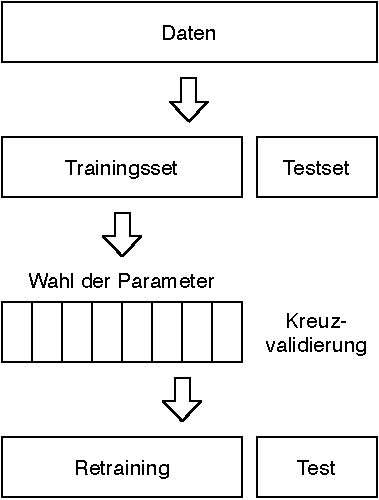
\includegraphics[scale=1]{pic/validation-ablauf.pdf}
		\caption{Ablauf von Training und Validierung}
		\label{fig:validation-ablauf}
	\end{figure}
	
	Um die Auswahl für ein Modell treffen zu können, werden Evaluationsmetriken benötigt. Für diese werden im Folgenden die englischen Bezeichnungen verwendet, da diese auch im Deutschen geläufiger sind.
	
	Vor allem für die Bewertung binärer Klassifikationen gibt es verschiedenste Metriken, die die richtigen und falschen Klassifikationen miteinander gewichten. Dafür wird bei positiv klassifizierten Datenpunkten zwischen Richtig-Positiven TP und Falsch-Positiven FP unterschieden; bei den negativ klassifizierten zwischen Richtig-Negativen TN und Falsch-Negativen FN. Eine Darstellung dieser vier nennt man Confusion Matrix. Diese ermöglicht eine erste Einschätzung der Fehlerverteilung. Ein häufig verwendetes und einfaches Gütemaß ist die Accuracy $\text{ACC} = \frac{TP + TN}{TP + TN + FN + FP}$, die allerdings bei ungleich großen Klassen problematisch ist, da eine hohe Genauigkeit erreicht wird, wenn immer die größere Klasse vorausgesagt wird. In diesem Fall kann auch die Balanced Accuracy verwendet werden, die dieses Ungleichgewicht einbezieht:
	\[
		\text{balanced-accuracy} = \frac{1}{2}\left( \frac{TP}{TP + FN} + \frac{TN}{TN + FP}\right).
	\]
	 Bei der Precision, auch Positive Predictive Value, $\text{PPV} = \frac{TP}{TP + FP}$ werden falsch-positive Klassifikationen \glqq bestraft\grqq{}; beim Recall, der \acl{TPR} $\text{TPR} = \frac{TP}{TP + FN}$, auch Sensitivity genannt, falsch-negative Klassifikationen. Letztere werden oft in einem Maß zusammengefasst, dem F1-Score, der das harmonische Mittel aus beiden bildet:
	\[
		F_1 = 2 \cdot \frac{\text{PPV} \cdot \text{TPR}}{\text{PPV} + \text{TPR}}.
	\]
	
	Eine weitere Möglichkeit, die Qualität eines binären Klassifikators zu evaluieren, ist die \ac{ROC} Kurve, bei der die \ac{TPR}, also der Recall, und die \ac{FPR} gegeneinander aufgetragen werden und so den Kompromiss zwischen \ac{TPR} und \ac{FPR} abhängig vom Schwellwert zeigt. Die Fläche unter dieser Kurve, die \ac{AUC}, beschreibt, wie gut das Modell die beiden Klassen trennt. Eine perfekte Trennung führt zu $\text{AUC} = 1$.
	
	Bei einer Regression werden üblicherweise der \ac{MAE} oder der \ac{MSE} betrachtet, die die Größe des Fehlers von dem vorhergesagten $\hat{y}$ im Vergleich zur Zielgröße $y$ ausdrücken und wie folgt berechnet werden:
	\begin{align*}
		\text{MAE}(y, \hat{y}) &= \frac{1}{n_{\text{samples}}} \sum_{i=0}^{n_{\text{samples}}-1} \left| y_i - \hat{y}_i \right| \\
		\text{MSE}(y, \hat{y}) &= \frac{1}{n_\text{samples}} \sum_{i=0}^{n_\text{samples} - 1} (y_i - \hat{y}_i)^2		
	\end{align*}
	
	Die Auswahl der betrachteten Metriken ist von dem vorliegenden Problem abhängig. %TODO: mehr Inhalt in Sätzen ist cool

	\subsection{Lernmodelle und deren mathematischer Hintergrund}
	
		Es gibt eine Vielzahl von Modellen des maschinellen Lernens, von denen eine Auswahl in dieser Arbeit betrachtet und vorgestellt wird. Alle verallgemeinern eine Verteilung von Trainingsdaten und haben das Ziel, eine Funktion $g$ zu finden, die $f$ approximiert und mit der die Zielgröße $y$ vorhergesagt werden kann. Bei einer Klassifikation sollen die verschiedenen Klassen möglichst genau separiert und bei einer Regression der Wert möglichst genau vorhergesagt werden. Diese Funktion wird auch Entscheidungsfunktion genannt und minimiert eine gewählte Kostenfunktion, die beschreibt, wie sehr die Vorhersagen von der Zielgröße abweichen. Bei linearen Modellen beispielsweise ist die Vorhersage mit $\hat{y}_i = \theta x_i$ eine lineare Kombination der gewichteten Merkmale für Datenpunkt $x_i \in X$. $\hat{y}_i$ kann dabei entweder direkt die Vorhersage eines Wertes sein oder genutzt werden, um eine Klassenzugehörigkeit zu ermitteln. Bei einer binären Klassifikation kann dafür beispielsweise die Signum- oder die logistische Funktion mit einem Schwellwert genutzt werden. Die genutzte Funktion wird auch Aktivierungsfunktion genannt. Die Parameter der Entscheidungsfunktion, in diesem Fall die Koeffizienten des Merkmalsvektors, werden im Nachfolgenden allgemein $\theta$ genannt. Sie sind der Teil der Entscheidungsfunktion, der von den Daten gelernt werden muss.
		
		Während des Trainings werden die besten Parameter $\theta$ ermittelt. Dafür wird eine Funktion benötigt, die ausdrückt, wie gut das Modell den Trainingsdaten angepasst ist. Diese besteht allgemein aus zwei Teilen: der Kostenfunktion $L$ und der Regularisierung $\Omega$:
		
		\[
			C(\theta)= L(\theta) + \Omega(\theta)
		\]
		
		Als Kostenfunktion wird vor allem für Regressionsprobleme häufig der \ac{MSE} verwendet. Bei binären Klassifikationsproblemen kann aber beispielsweise auch die Anzahl der falschen Klassifikationen verwendet werden. Die Regularisierung kontrolliert die Komplexität des Modells, um Overfitting zu vermeiden. Das Ziel des Trainings ist es demnach, die Anpassung des Modells zu optimieren, also $C$ zu minimieren. Dieses Minimierungsproblem wird abhängig von dem verwendeten Modell gelöst. Bei einer linearen Regression beispielsweise kann die Methode der kleinsten Quadrate verwendet werden, um die Fehlerquadrate zu minimieren, da eine Regularisierung bei einem linearen Modell nicht nötig ist. Der Gewichtungsvektor $\theta$ kann hier durch direktes Auflösen berechnet werden:
		\[
			\argmin_{\theta} \sum_{i=1}^{n} (\theta^T x_i - y_i)^2
			\Rightarrow \theta = (X^T X)^{-1} X^Ty
		\]
		
		Bei komplexeren Minimierungsproblemen ist die Methode kleinster Quadrate nicht ausreichend und es werden andere Methoden zur Fehlerminimierung benötigt. Eines davon ist das Gradientenabstiegsverfahren, bei dem in jedem Schritt die Ableitung der Kostenfunktion nach jedem der Gewichte berechnet wird und der Schritt gewählt wird, der die Funktion am stärksten minimiert.
		
		Eine andere Möglichkeit ist, nicht linear separierbare Daten mit dem sogenannten Kerneltrick linear separierbar zu machen, statt nicht-lineare, komplexere Verfahren zu verwenden. Dabei wird durch Ersetzen des Skalarproduktes implizit der Variablenraum transformiert. Ein Beispiel ist der Gaußsche RBF-Kernel, wobei RBF für radial basis function steht. Sind $x$ und $x'$ Merkmalsvektoren, ist der RBF-Kernel wie folgt definiert:
		\[
			K_{RBF} (x, x\prime) := \text{exp}(-\gamma \|x - x\prime\|^2) \text{ mit } \gamma > 0
		\]
		In der Transformation werden alle Nicht-Linearitäten berücksichtigt, wodurch anschließend Linearität möglich ist. %TODO: besser formulieren
		
		Im Folgenden werden die in dieser Arbeit genutzten Modelle näher vorgestellt. Die Nachimplementierung von existierenden Algorithmen umfasst außerdem drei Modelle, die hier nicht detailliert vorgestellt werden: die \ac{SVM}, die \ac{LDA} und das \ac{MLP}. Wichtig für die Einordnung ist, dass es sich bei \ac{LDA} und \ac{SVM} um zunächst lineare Modelle handelt und die \ac{SVM} häufig mit dem Kerneltrick verwendet wird, um die Daten zu transformieren. Beim \ac{MLP} handelt es sich um ein Neuronales Netz, das Nichtlinearität ermöglicht.

	
		\subsubsection{Classification And Regression Trees}
		
		\ac{CART} sind nicht-lineare Modelle, die einem Binärbaum entsprechen. Sie können sowohl für Regression als auch für Klassifikation verwendet werden. Zwar sind sie hinsichtlich ihrer Performance oft anderen Lernmodellen unterlegen, werden aber als Teil von komplexeren Modellen genutzt und haben den Vorteil, sehr gut nachvollziehbar zu sein. Im Gegensatz zu vielen anderen Modellen benötigen sie keine Normalisierung der Merkmale. Es wird ein Pfad in einem Baum durchlaufen, indem an jedem Knoten unterschieden wird, ob ein bestimmtes Merkmal über oder unter einem Schwellwert liegt. Die Kostenfunktion bei einer Regression ist in der Regel der \ac{MSE}. Für die Kostenfunktion einer Klassifikation wird häufig die \glqq{}Reinheit\grqq{} eines Knoten $m$ gemessen. Sie beschreibt, wie deutlich die Mehrheit einer einzelnen Klasse in $m$ ist.
		
		Für den Aufbau eines \ac{CART} wird häufig das zu den greedy Algorithmen gehörende rekursive binäre Teilen verwendet. Hierbei wird ein Baum von der Wurzel zu den Blättern hin aufgebaut. In jedem Schritt wird das Merkmal gewählt, mit dem sich die Daten zu diesem Zeitpunkt am besten separieren lassen und der Schwellwert ermittelt. Abbruchkriterien sind unter anderem eine maximal erlaubte Tiefe oder eine Mindestanzahl von Datenpunkten in einem Blatt. Wenn diese zu viel Spielraum erlauben, neigen Bäume zum Overfitting.
		
		\subsubsection{Random Forest}
		
		Ein Zusammenschluss aus mehreren unkorrelierten Bäumen wird \acf{RF} genannt. Jeder dieser Bäume ist ein eigenständiges Modell, das ein Ergebnis liefert. Aus der Menge der Einzelergebnisse wird das endgültige Ergebnis ermittelt. Dadurch wird ein Teil der Nachvollziehbarkeit von Bäumen gegen eine bessere Generalisierung eingetauscht. Die einzelnen Bäume werden zufällig erzeugt, indem für jeden Baum $n$ zufällige Datenpunkte ausgewählt werden. Von $M$ Merkmalen werden nun $m \ll M$ ebenfalls zufällig gewählt, die als Kriterium für den Aufbau des Baumes verwendet werden. Der darauf folgende Aufbau des Baumes entspricht dem zuvor beschriebenen. Bei einer Klassifikation ist das endgültige Ergebnis je nach Implementierung ein Mehrheitsentscheid oder eine Kombination aller Wahrscheinlichkeiten; bei einer Regression der Durchschnitt aller Werte.
		
		Ein Random Forest hat gegenüber anderen Modellen den Vorteil, dass er sehr schnell trainiert und somit sehr effizient für große Datenmengen ist. Gleichzeitig kann das Ergebnis relativ einfach nachvollzogen werden.
		
		\subsubsection{Gradient Boosted Trees}
		
		Auch ein Gradient Boosted Tree kombiniert mehrere einfache Bäume. Im Gegensatz zum \ac{RF} hängt beim Gradient Boosted Tree jeder Baum von früheren Bäumen ab. Gestartet wird mit einem Baum, auf dessen Ergebnissen aufgebaut wird. Das endgültige Ergebnis wird auch hier aus der Menge an einzelnen Ergebnissen ermittelt, aber folgende Bäume konzentrieren sich jeweils darauf, die Schwächen der schon erzeugten Modelle auszugleichen.
		
		Auch Gradient Boosted Trees ermöglichen eine nachvollziehbare Entscheidung. Meist erreichen sie etwas bessere Ergebnisse als die einfacheren \acl{RF}s.

\section{Medizinische Grundlagen}\label{med-grundlagen}

Die vorliegende Arbeit beschäftigt sich mit der Beurteilung der Signalqualität in ballistokardiographischen Signalen. Zum Verständnis der gemessenen Vorgänge und der Problematik in Bezug auf die Signalqualität und dessen Beurteilung ist grundlegendes medizinisches Wissen über die gemessenen Vorgänge und messtechnisches Verständnis nötig. Aufgrund dessen wird hier eine kurze Übersicht über die medizinischen Grundlagen gegeben.

	\subsection{Kardiorespiratorisches System}
	
	Das kardiorespiratorische System (zusammengesetzt aus \textit{kardìa}, deutsch \glq Herz\grq{} und \textit{respiratio}, deutsch \glq Atmung\grq) setzt sich aus zwei Teilsystemen zusammen, dem kardiovaskulären und dem respiratorischen System, die zusammen die Versorgung der Organe mit Sauerstoff sicherstellen.
	
	Das kardiovaskuläre System umfasst das Herz, die Arterien und die Venen. In einem Zyklus wird das sauerstoffreiche Blut von der linken Herzkammer durch die Arterien zu den Organen gepumpt, wo sich der Sauerstoff zur Versorgung dieser vom Blut löst. Die Venen transportieren das nun kohlstoffdioxidreiche Blut in die rechte Herzkammer. Von dort wird es zur Lunge geführt, mit Sauerstoff angereichert und in die linke Herzkammer geleitet. Von dort beginnt der Vorgang von Neuem. Die Herzfrequenz ist hierbei ein relevanter messbarer Vitalparameter.
	
	Ein Herzschlag selbst besteht aus zwei Phasen: einer füllenden und einer auswerfenden Phase. Während der Diastole, der Erschlaffungs- und Bluteinströmungsphase, füllen sich die Herzkammern mit Blut. Diese Phase endet mit dem Schließen der Herzklappen und die Systole beginnt. Die Systole ist die Anspannungs- und Blutausströmungsphase: Die Herzklappen öffnen sich durch Kontraktion des Herzmuskels und das Blut kann ausströmen.
	
	Das respiratorische System umfasst die Lungen und den Lungenkreislauf. In einem Atemzyklus wird durch gezielte Muskelbewegungen Luft aus der Umgebung eingeatmet. Mit dem eingeatmeten Sauerstoff wird sauerstoffarmes Blut angereichert und anschließend die nun sauerstoffarme Luft ausgeatmet. In diesem Zusammenhang ist der Vitalparameter der Atemfrequenz messbar.

	\subsection{Übersicht Messtechniken}
	
	Zur Untersuchung der in dieser Arbeit betrachteten \acf{BKG} wird diese oft mit anderen Messmethoden als Referenz aufgenommen. Im Folgenden werden diese zur Einordnung kurz vorgestellt. \ac{BKG} selbst wird im nächsten Abschnitt separat betrachtet.
	
	Die \acf{EKG} zeichnet die elektrischen Aktivitäten des Herzmuskels auf, indem mit mehreren Elektroden die Spannungsänderung gemessen wird. Hier ist die Herzfrequenz sehr gut ablesbar.
	
	Die \acf{PPG} ist ein optisches Messverfahren, bei dem die Menge des von der Haut reflektierten bzw. transmittierten Lichtes gemessen wird. Dadurch kann die Änderung des Blutvolumens gemessen werden; die Lichtmenge nimmt bei Durchlaufen einer Pulswelle durch die Arterie deutlich ab. Dieses Signal bietet Rückschluss auf Atmung und Herzschlag. % TODO: evtl. rausnehmen
	
	Oft gemeinsam mit dem \ac{BKG} betrachtet wird die \acf{SKG}, bei der die Vibration der Wand des Brustkorbs, die durch den Herzschlag entsteht, aufgezeichnet wird. Aufgrund von fehlenden einheitlichen Definitionen wird in der Literatur teils auch der Begriff \ac{BKG} für \ac{SKG} genutzt.\footcite[Vgl.][]{Inan2015}

	\section{Ballistokardiographie}\label{ballistokardiographie}
	
	Im Folgenden wird die \acl{BKG} eingeführt. Diese Einführung beinhaltet den medizinischen und technischen Hintergrund, das Einsatzgebiet und die Signaleigenschaften.
	
	\subsection{Medizinischer und technischer Hintergrund}
	
	Ballistokardiographie (zusammengesetzt aus altgriechisch \textit{ballein}, deutsch \glq werfen\grq, \textit{kardía}, deutsch \glq Herz\grq{} und \textit{graphein}, deutsch \glq schreiben\grq) ist die graphische Darstellung der wiederholten, durch den Herzschlag verursachten Bewegungen des menschlichen Körpers. Erstmals schon im 19. Jahrhundert beobachtet\footcite[Vgl.][]{Gordon1877}, ermöglicht der technische Fortschritt in der Sensortechnik heute aussagekräftige Messungen. Das \ac{BKG} liefert durch die Aufzeichnung von zirkulierendem Blut und mechanischer Herzaktivität Informationen über die Gesamtleistung des kardiovaskulären Systems.\footcite[Vgl.][]{Pinheiro2010} Konkret gemessen wird eine Massenbewegung, die durch die schnelle Beschleunigung des Blutes entsteht, wenn es während des Herzschlages durch die großen Arterien bewegt wird: Bei der Verteilung des Blutes in die peripheren Blutgefäße verschiebt sich das Zentrum der Körpermasse in Richtung der Füße und während der atrialen Systole Richtung Körpermitte. Die \ac{BKG}-Wellenform entsteht durch diese Schwerpunktverschiebung.
	
	Die Messung dieser Bewegung ist mit verschiedenen Sensortypen, die z.\,B. hydraulisch oder elektromechanisch auf Druck reagieren, möglich. Sensoren können unter anderem in Waagen, Stühlen und Betten eingebaut werden. Besonders bei im Bett gemessenen Signalen kann oft nicht klar zwischen \ac{SKG} und \ac{BKG} unterschieden werden, da sich myokardiale Vibrationen und Massverschiebungen durch den Blutfluss überlagern. Diese gemischten Signale werden in der Literatur teils auch als \textit{cardiac vibration signals} bezeichnet.\footcite[Vgl.][]{Bruser2013} Da im Bereich der Signalverarbeitung oft nicht zwischen reinem \ac{BKG} und gemischten Signalen unterschieden wird, wird dies in der vorliegenden Arbeit ebenfalls nicht. %TODO: wird nach dem Komma ersetzen
	
	Verschiedene Studien kommen zu unterschiedlichen Ergebnissen bezüglich der Frage, welchen kardiovaskulären Ursprung die einzelnen Signalteile haben. Aufgrund dessen gestaltet sich die detaillierte Interpretation des \ac{BKG}-Signals als schwierig. Da es neben Informationen zur \ac{HR} und \ac{HRV} ein genauerer Indikator für das Alter des Herzens als Lebensalter ist, hat es trotzdem klinische Relevanz. Außerdem lassen sich durch abnormale Ballistokardiogramme Herzerkrankungen voraussagen, bevor Symptome auftreten. Besonders bei älteren Personen sind diese also eine wichtige Warnung.\footcite[Vgl. zu diesem Absatz][]{Pinheiro2010}
	
	\subsection{Einsatzgebiet}
	
	Durch diese Beschreibung wird deutlich, dass \ac{BKG} anders als die sehr bekannte \ac{EKG} ist. Der entscheidende Vorteil der \ac{BKG}s liegt darin, dass kein einschränkender Körperkontakt durch z.\,B. aufgeklebte Elektroden nötig ist: Es lässt sich in Alltagsgegenständen wie Stühlen aber vor allem auch Betten implementieren, ohne dass es während der Messung zu Einschränkungen im alltäglichen Leben kommt oder medizinisches Fachpersonal anwesend sein muss. Damit gehört es zu den \textit{unobtrusive} Messmethoden und eignet sich gut zur Langzeit- und Trendbeobachtung des Gesundheitszustandes - sowohl im klinischen Kontext als auch Zuhause. Besonders für Patient*innen mit chronischen Krankheiten und zur Früherkennung krankhafter Veränderungen bietet eine gesundheitliche Überwachung von Zuhause großes Potential.\footcite[Vgl.][]{Inan2015} Je nach Aufbau des Messsystems verändert sich auch die Art der Informationen, die aus dem \ac{BKG}-Signal gewonnen werden können. Sehr genaue, kontrolliert aufgenommene \ac{BKG}-Signale ermöglichen eine aussagekräftige Analyse der Morphologie wobei beispielsweise in Betten eingebautes \ac{BKG} zunächst nur Aussagen zu Herzrate und Herzratenvariabilität bietet. Zusätzlich zu Informationen der Herzaktivitäten ermöglichen Bettsysteme aber auch Informationen über das allgemeine Aktivitätslevel und somit auch über die Schlafqualität. \footcite[Vgl.][]{Bruser2011} In dieser Arbeit wird es um die Aufzeichnung von \ac{BKG}-Signalen in Betten gehen. Der Aufbau eines solchen Bettsystems ist in Abbildung \ref{fig:bcgbed} gezeigt.
	
	 \begin{figure}[H]
	 	\centering
		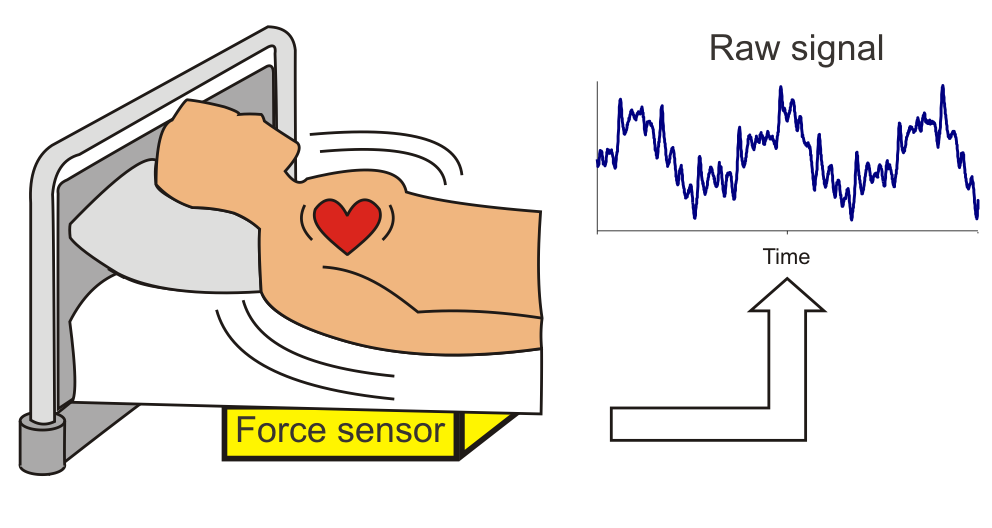
\includegraphics[width=0.7\textwidth]{pic/bcgBed.png}
		\caption[Übersicht über die Funktionsweise eines allgemeinen im Bett eingebetteten \ac{BKG}-Systems]{Übersicht über die Funktionsweise eines allgemeinen im Bett eingebetteten \ac{BKG}-Systems.\protect\footnotemark}
		\label{fig:bcgbed}
	\end{figure}
	\footnotetext{Entnommen aus \cite{Bruser2011}}
	
	Allerdings ergeben sich neben diesen umfassenden Möglichkeiten auch Nachteile gegenüber konventionellen Messmethoden. Die größte Herausforderung ist eine stark variierende Signalqualität, die sich durch das unkontrollierte Umfeld und die Art der Messung ergibt.

	\subsection{Signaleigenschaften}
	
	Das gemessene \ac{BKG}-Signal setzt sich aus Herzaktivitäten, Atmungsaktivitäten und Körperbewegungen zusammen. Gegebenenfalls wird es noch durch Störungen der Messung beeinflusst. Bei einer gesunden Person ohne Störeinflüsse wird die in Abbildung \ref{fig:bcgwaveform} abgebildete Wellenform erwartet. Diese Idealform lässt sich in 3 Gruppen unterteilen: Die präsystolische, wobei diese häufig nicht beachtet wird, die systolische und die diastolische Gruppe. Die mit H bis K markierten Extremwerte gehören bei dieser Unterteilung zur systolischen Gruppe, die Wellen L bis N zur diastolischen Gruppe. Die präsystolische Gruppe, die aus den Wellen F und G besteht, ist in hier nicht abgebildet. I und J werden auch als \textit{ejection waves} bezeichnet. In Bezug auf andere Messmethoden ist zu bemerken, dass die H-Welle nahezu synchron mit dem ersten Herzgeräusch ist. Der Abstand des R-Peaks, des Hochpunkts eines \ac{EKG}s, zur H-Welle variiert im Bereich von \numrange{0,2}{0,3} Sekunden.\footcite[Vgl.][]{DELALLA1950} Die Amplitude der Wellen ohne Störeinflüsse ist hauptsächlich abhängig von dem Herzzeitvolumen, der Herzkraft und der Geschwindigkeit des Auswurfs.\footcite[Vgl.][]{Pinheiro2010}
	
	\begin{figure}[H]
		\centering
		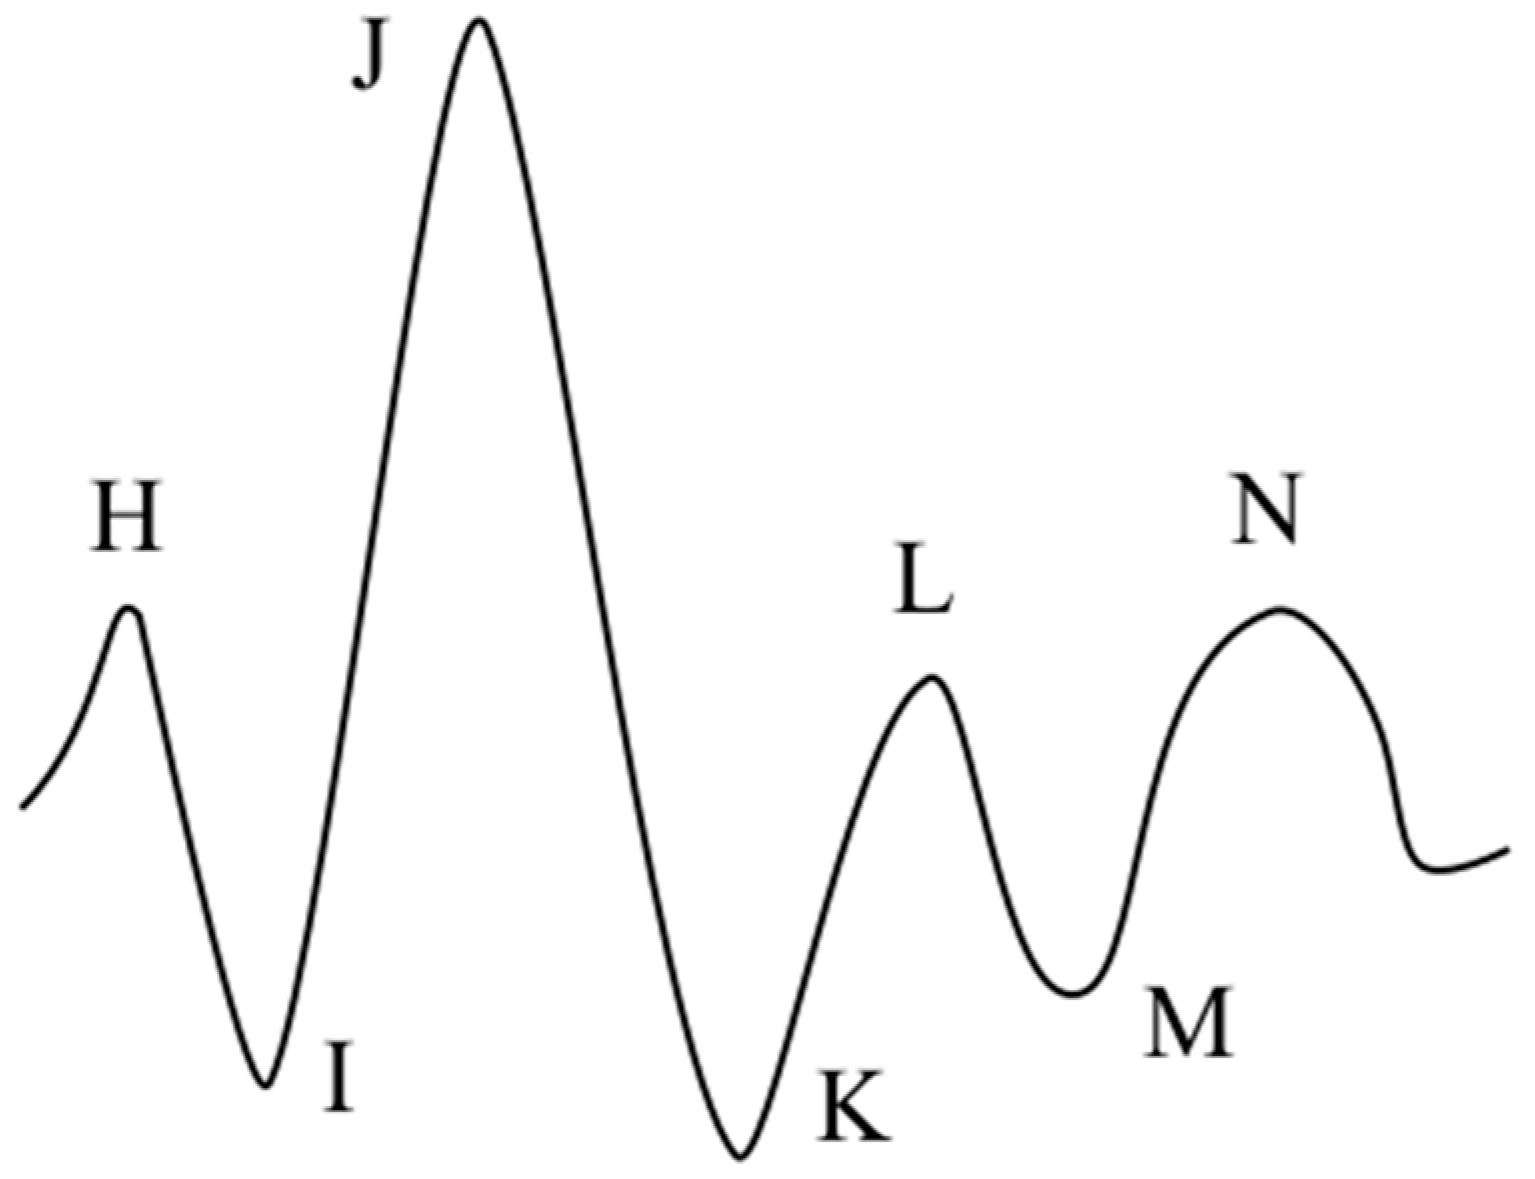
\includegraphics[width=0.7\textwidth]{pic/bcgWaveform.png}
		\caption[Beispiel eines typischen \ac{BKG}-Signals mit Nomenklatur]{Beispiel eines typischen \ac{BKG}-Signals mit Nomenklatur\protect\footnotemark}
		\label{fig:bcgwaveform}
	\end{figure}
	\footnotetext{Entnommen aus \cite{Albukhari2019} nach \cite{Starr1939}.}
	
	Im Idealfall wird zwar die oben beschriebene Wellenform erwartet, bei der die Wellen H bis L eine deutliche W-Form bilden, allerdings ist es trotz dieser typischen Form selten, dass alle nicht-systolischen Komponenten sichtbar sind.\footcite[Vgl.][]{Pinheiro2010} Es gibt eine starke Variation der Signalmorphologie sowohl zwischen als auch innerhalb von Individuen. Der größte Einfluss ergibt sich durch die verwendeten Sensoren und die Position der Person, also zum Beispiel ob im Stehen, Sitzen oder Liegen gemessen wird.\footcite[Vgl.][]{Sadek2019} Es gibt Studien, die zeigen, dass die intraindividuelle Varianz über serielle Messungen hinweg niedrig ist.\footcite[Vgl.][]{Inan2015} Allerdings gilt das nicht, wenn sich die Position der Person verändert. Hierbei reicht es schon, wenn die Person in Rückenlage statt Seitenlage liegt.\footcite[Vgl.][]{Bruser2011} Aufgrund dieser Variationen in der Signalmorphologie wurden schon in den 1950er Jahren drei Achsen für die Aufzeichnung des \ac{BKG}s definiert: Die longitudinale (Kopf-Fuß), die transversale (Seite-Seite) und die dorsoventrale (Rücken-Brust).\footcite[][Vgl.]{Bruser2011, Inan2015} Zu Beginn maßen die meisten Systeme entlang der longitudinalen Achse, die z.\,B. der Messung auf einer Waage entspricht. \textit{Unobtrusive} Messsysteme, wie die hier betrachtete Messung in Betten, messen entlang einer Kombination der transversalen und der dorsoventralen Achse - abhängig von der Position der Person. Besonders diese Kombination sorgt für eine große intra- und individuelle Variation des Signals. Abbildung \ref{fig:bcg2postures} verdeutlicht dies durch den direkten Vergleich von \ac{BKG}-Aufzeichnungen zweier Herzschläge von 2 Personen. Bei jeder dieser beiden Personen wurde in zwei verschiedenen Positionen gemessen.\footcite{Bruser2011} Auch der Ursprung des Signals ist abhängig von der Messachse. Bei longitudinal gemessenem \ac{BKG} ist der Einfluss des Herzzeitvolumens schon seit 1929 beobachtet.\footcite[Vgl.][]{Starr1939} Im Gegensatz dazu ist der Ursprung des in Betten gemessenen \ac{BKG}-Signals nicht genau bekannt. Das liegt unter anderem daran, dass mechanische Komponenten wie z.\,B. die Matratze einen schwer zu modellierenden Einfluss haben.
	
	\begin{figure}[H]
		\centering
		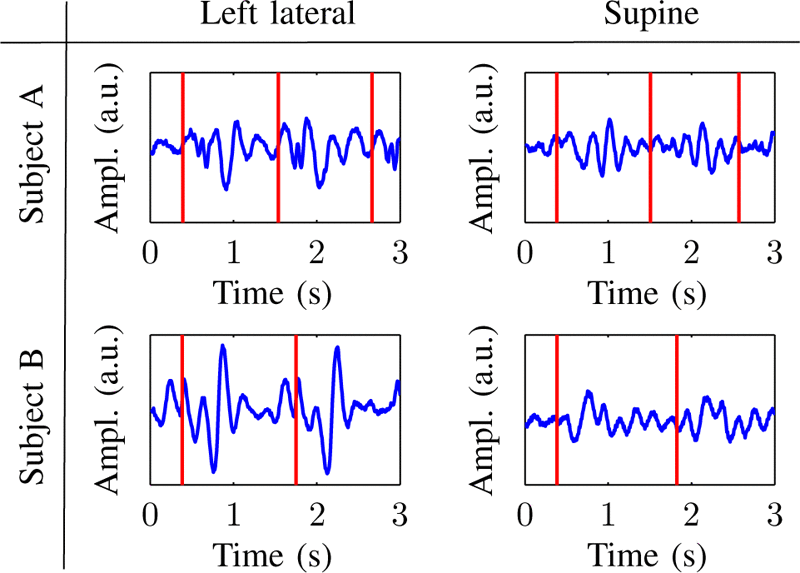
\includegraphics[width=0.7\textwidth]{pic/bcg2postures.png}
		\caption[\ac{BKG}-Aufnahmen in Rücken- und Seitenlage]{Hochpass-gefilterte \ac{BKG}-Aufnahmen von zwei Herzschlägen zwei verschiedener Personen, jeweils in Rücken- und Seitenlage gemessen. Die vertikalen Linien markieren die R-Peaks der EKG-Referenz.\protect\footnotemark}
		\label{fig:bcg2postures}
	\end{figure}
	\footnotetext{Entnommen aus \cite{Bruser2011}.}
	
	Neben Einflüssen der verwendeten Messachse und der Körperposition beeinflusst auch die Atmung die Signalform. Normale Atmung beeinflusst die Amplitude der \textit{ejection waves} I und J. Bei Atemstillstand dagegen werden die H und J Wellen verzerrt. Auch bei einer gesunden, sich nicht bewegenden Person, die ihre Atmung kontrolliert, wird kein exakt Schlag für Schlag reproduzierbares Signal erzeugt werden.\footcite[Vgl.][]{Pinheiro2010} Von \citeauthor{Zink2017} werden die Einflüsse der Atmung in der vertikalen Achse eines dorsoventralen \ac{BKG}s als große Schwingungen einer Wellenlänge von fünf bis zehn Sekunden beschrieben. Innerhalb dieser sind kleinere Schwingungen mit höherer Frequenz sichtbar, die jedoch keiner bestimmten Sequenz folgen.\footcite[Vgl.][]{Zink2017} Zusätzlich zu dieser schon beschriebenen Variabilität kommt es sehr leicht zum Entstehen von Artefakten. Ursprung ist entweder das Messsystem selbst oder Körperbewegungen. Insgesamt führt Bewegung der Patient*innen, auch die der Atmung, zu einem \textit{baseline drift}. Stärkere Bewegungen führen zu einer Massenverschiebung, die um ein Vielfaches größer als die gemessenen Vorgänge ist. Aufgrund dessen führt sie immer dazu, dass das Signal stark verzerrt oder sogar vollständig überlagert wird.

	
	Besonders im Vergleich zu anderen kardiorespiratorischen Signalen wie dem \ac{EKG} und \ac{PPG} wird deutlich, dass \ac{BKG}-Signale auch in konsekutiven Messungen deutlich variabler sind. Abbildung \ref{fig:variabilitaet} zeigt dies am Beispiel von \ac{BKG}-Aufnahmen eines im Bett integrierten Messsystems im Vergleich zum parallel aufgenommenen \ac{EKG}. Es zeigt sich, dass selbst nach Entfernung von Überlagerungen von Atmung  und Bewegung das \ac{BKG}-Signal eine höhere Variabilität in Bezug auf Amplitudenhöhe, Reihenfolge der Extremwerte und der gesamten Form aufweist.\footcite[Vgl.][]{Zink2017} Es wird allerdings angenommen, dass aufeinander folgende Herzschläge sich ähneln.\footcite[Vgl.][]{Bruser2013} Diese Eigenschaft wird Selbstähnlichkeit genannt. \citeauthor{Bruser2013} nennen als eine mögliche Ausnahme den Fall, dass ein unregelmäßiger Herzschlag mit sehr niedrigem Schlagvolumen einem regulären Herzschlag folgt. In dem Fall ist es möglich, dass die Amplitude im Vergleich so klein ist, dass sie verdeckt wird. Dies ist z.\,B. bei Vorhofflimmern möglich. Eine Untersuchung von \citeauthor{Rosales2012} zeigt dieses Verhalten der Selbstähnlichkeit nicht bei den kleineren Extremwerten die den Hochpunkt J umgeben. Dass die Ähnlichkeit um J am größten ist, zeigt auch Abbildung \ref{fig:variabilitaet}.
	
	\begin{figure}[H]
		\centering
		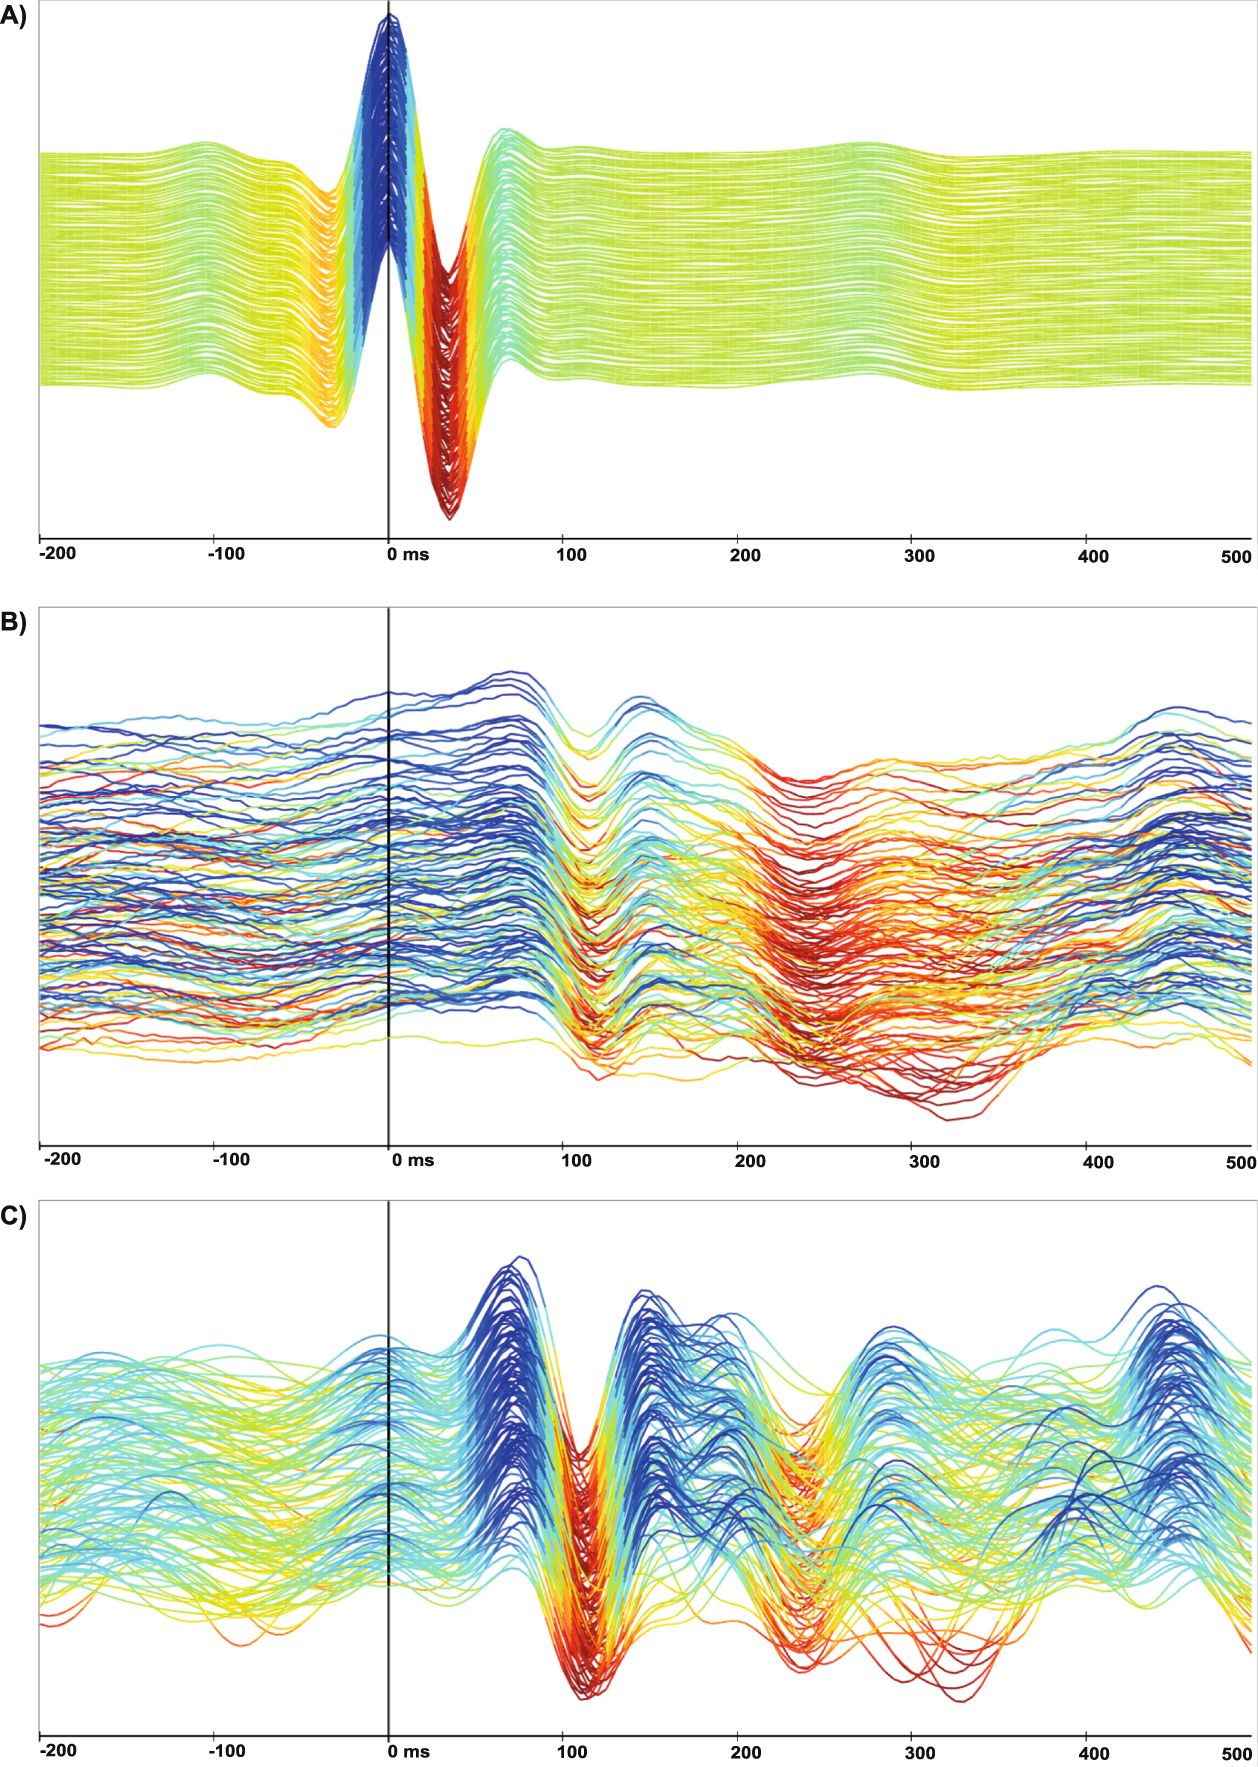
\includegraphics[width=0.6\textwidth]{pic/Variabilitaet.jpg}
		\caption[Visualisierung der Variabilität des \ac{BKG}-Signals]{Diagramm aus 128 konsekutiven Herzschlagen im EKG (A) und BKG (B,C), segmentiert durch das EKG. Die Farben dienen der besseren Visualisierung der Amplituden. (A) EKG-Signal; (B) BKG-Signal mit Überlagerungen durch Atmung und Bewegung; (C) \ac{BKG}-Signal ohne Bewegungsartefakte und Atmung.\protect\footnotemark}
		\label{fig:variabilitaet}
	\end{figure}
	\footnotetext{Entnommen aus \cite{Zink2017}.}
	
	
	Zusammengefasst lässt sich sagen, dass es sich bei ballistokardiographischen Signalen um nichtstationäre Signale handelt, deren Ursprung nicht genau bekannt ist. Die Signalform wird von der Messachse, der Position und Körperhaltung der Proband*innen und dem Messsystem selbst beeinflusst. Besonders bei dem hier im Fokus liegenden Anwendungsfall Bett kommt es sowohl durch die unkontrollierbare Umgebung als auch die Signaleigenschaften selbst zu einer starken Variation der Morphologie und vielen Artefakten im Signal. Trotz dieser Einschränkungen ist die \acl{BKG} eine Messtechnik, die sich einfach \textit{unobtrusive} in den Alltag einbauen lässt und Aussagen über die \acl{HR} und die \acl{HRV} ermöglicht.


\chapter{Ergebnisse und Ausblick}\label{Ergebnis}

\section{Ergebnisse}


\section{Ausblick}






%***********************************************************
%* Anhänge			 									   *
%***********************************************************
%\addcontentsline{toc}{chapter}{Anhang}
%\appendix
%\input{./app/Dateiname}
%\chapter{Datenblätter}
%\begin{enumerate}
%      \item Datenblatt 1
%      \item Datenblatt 2
%\end{enumerate}


%***********************************************************
%* Quellenverzeichnis 									   *
%***********************************************************
\clearpage
\printbibliography[heading=bibintoc]
%\bibliographystyle{plainnat}
%\bibliography{./bib/quellen}

\end{sloppypar}
\end{document}
